\documentclass[a4paper]{article}
\usepackage{a4wide}
\usepackage{tikz}

\pagestyle{empty}

\begin{document}
\begin{center} \Huge
  Vierkantsvergelijkingen \\
  \large (a.k.a.\ tweedegraadsvergelijkingen)
\end{center}

Een tweedegraadsvergelijking is een vergelijking die kan geschreven worden in de vorm
\[
  a \cdot x^2 + b \cdot x + c = 0
\]

Indien men ze uittekent krijgen we bijvoorbeeld
\begin{center}
  \begin{tabular}{ccc}
    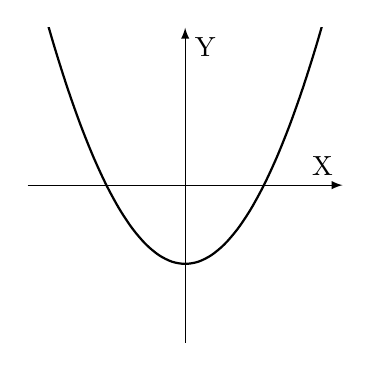
\begin{tikzpicture}[domain=-2:2,
                        axis/.style={thin,-latex}]
      \begin{scope}
        \path[clip] (-2,-2) rectangle (2,2);
        \draw[axis] (-2,0) -- (2,0) node[at end,above,anchor=south east] {X};
        \draw[axis] (0,-2) -- (0,2) node[at end,right,anchor=north west] {Y};
        \draw[thick,smooth] plot (\x, \x*\x - 1);
      \end{scope}
    \end{tikzpicture}
    &
    \begin{tikzpicture}[domain=-2:2,
                        axis/.style={thin,-latex}]
      \begin{scope}
        \path[clip] (-2,-2) rectangle (2,2);
        \draw[axis] (-2,0) -- (2,0) node[at end,above,anchor=south east] {X};
        \draw[axis] (0,-2) -- (0,2) node[at end,right,anchor=north west] {Y};
        \draw[thick,smooth] plot (\x, \x*\x-2*\x+1);
      \end{scope}
    \end{tikzpicture}
    &
    \begin{tikzpicture}[domain=-2:2,
                        axis/.style={thin,-latex}]
      \begin{scope}
        \path[clip] (-2,-2) rectangle (2,2);
        \draw[axis] (-2,0) -- (2,0) node[at end,above,anchor=south east] {X};
        \draw[axis] (0,-2) -- (0,2) node[at end,right,anchor=north west] {Y};
        \draw[thick,smooth] plot (\x, 3*\x*\x + 5*\x + 2.5);
      \end{scope}
    \end{tikzpicture} \\
    $x^2 - 1$ & $x^2-2x+1$ & $6x^2+10x+5$ \\
  \end{tabular}
\end{center}

Een vierkantsvergelijking oplossen komt overeen met het zoeken van de snijpunten van de parabool
met de X-as. Op de derde figuur zie je dat het perfect mogelijk is dat er geen zulke snijpunten bestaan.
Om uit te kunnen maken of er weldegelijk snijpunten zijn, rekenen we eerst de discriminant uit.
Deze is gelijk aan (van buiten te kennen):
\[
  D = b^2 - 4 \cdot a \cdot c
\]
Het teken van $D$ heeft de volgende betekenis:
\begin{center}
  \begin{tabular}{cl}
    $D > 0$ & Er zijn twee verschillende oplossingen \\
    $D = 0$ & Er zijn twee gelijke oplossingen \\
    $D < 0$ & Er zijn geen oplossingen
  \end{tabular}
\end{center}
We rekenen de discriminanten uit van de voorbeelden:
\begin{itemize}
  \item Voorbeeld 1: $D = 0^2 - 4 \cdot 1 \cdot (-1) = 4$
  \item Voorbeeld 2: $D = (-2)^2 - 4 \cdot 1 \cdot 1 = 0$
  \item Voorbeeld 3: $D = 10^2 - 4 \cdot 6 \cdot 5 = 100 - 120 = -20$
\end{itemize}

Voorbeeld 3 heeft, zoals de grafiek het reeds aanduidt, geen oplossingen. Voorbeeld 2 toont hoe twee gelijke oplossingen
eruitzien: de parabool \emph{raakt} de X-as.

De discriminant vertelt ons of er snijpunten zijn; laten we nu de snijpunten ook zoeken. De formule hiervoor (van buiten te kennen):
\[
  x_{1,2} = \frac{-b \pm \sqrt{D}}{2a}
\]

We rekenen het uit voor de voorbeelden:
\begin{itemize}
  \item Voorbeeld 1: $x_1 = \frac{-0-\sqrt{4}}{2\cdot 1} = 1$, $x_2 = \frac{-0+\sqrt{4}}{2\cdot 1} = 1$
  \item Voorbeeld 2: $x = \frac{-(-2)-\sqrt{0}}{2\cdot 1} = 1$
\end{itemize}

\paragraph{Oefeningen}
Je kan je eigen oefeningen gemakkelijk opstellen als volgt: kies zelf getallen $x_1, x_2$ en $a$. De vergelijking
\[
  a \cdot (x-x_1)\cdot(x-x_2)=0
\]
heeft dan als oplossingen $x_1$ en $x_2$. Als je distributiviteit toepast, verkrijg je
\[
  a \cdot x^2 - a \cdot (x_1 + x_2) \cdot x + x_1 \cdot x_2 = 0
\]
Deze kan je dan oplossen op bovenstaande manier. Bijvoorbeeld, we nemen $x_1 = -1$, $x_2 = 1$ en $a = 1$.
We krijgen dat
\[
  1 \cdot (x - (-1)) \cdot (x + 1) = (x + 1) \cdot (x - 1) = x^2 - 1
\]
Deze komt schoon overeen met voorbeeld 1.

\end{document}

